% Moved transit constraints to Model.tex  -Scott

\section{Empirical Evaluation}
  
In this section we compare the solutions for traffic networks modeled as a QTM
before and after the introduction of a public transit network, and with both fixed control
and optimized control, w.r.t. to two evaluation criteria:
the quality of solutions and the amount of delay introduced by the transit.
%
%
% TODO \fnremark{FWT: I don't think that optimal is the best word here since
%we arbitrarily fixed a value of \DT[]. Also, there is the technical problem that
%Gurobi might not have found the true optimal.}
%
Specifically, we compare the quality of solutions based on the total travel time and we also
consider the third quartile and maximum of the observed delay distribution.
%
%% TODO(fwt): maybe define what we mean by optimal here, for instance
%
%For our experiments, we consider as optimal solution, the MILP solution of a
%QTM using small enough homogeneous \DT[] with unlimited computational
%resources.
%
Our hypothesis is that that by applying optimized signal control to the traffic,
we are able to nullify the impact of introducing a public transit, and with a quality 
and delay comparable to that before the transit was introduced.
%
In the remainder of this section, we present the traffic networks considered in
the experiments, our methodology, and the results.



\subsection{Networks}



\begin{figure}[t!]
\centering
%  trim={<left> <lower> <right> <upper>}
\subfigure[]{
\label{subfig:network1}
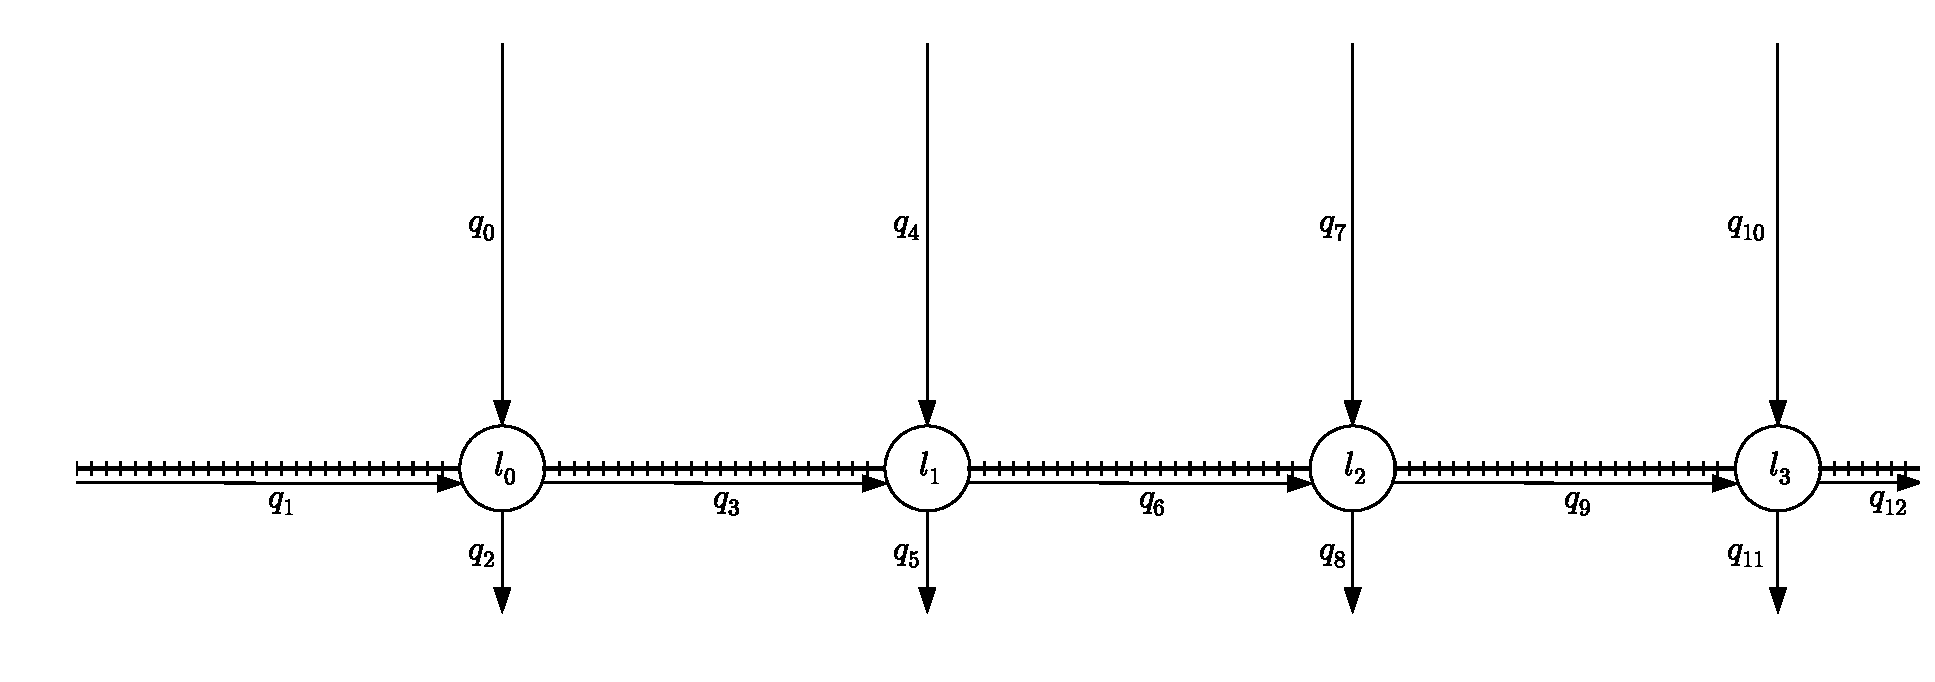
\includegraphics[width=0.47\textwidth]{network1.pdf}}
\subfigure[]{
\label{subfig:network2}
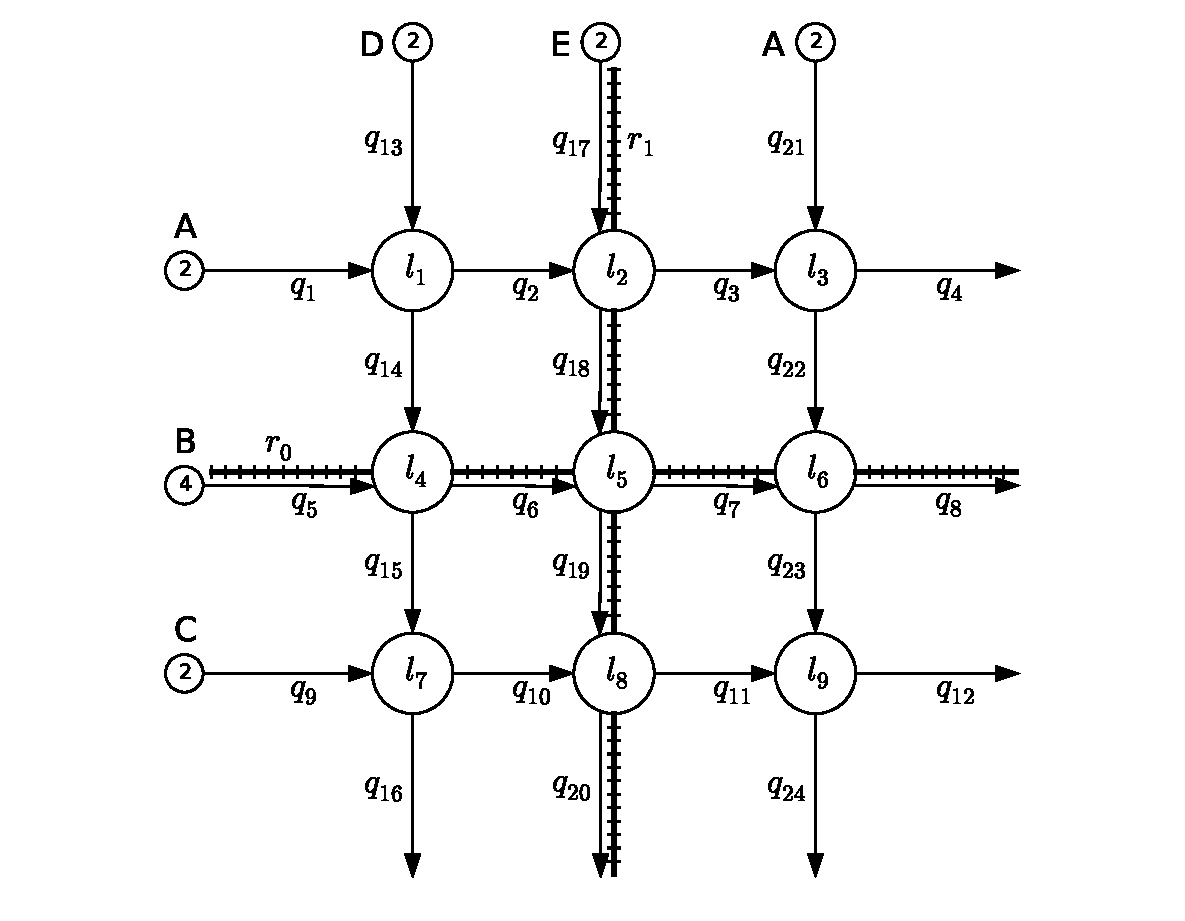
\includegraphics[width=0.40\textwidth]{network2.pdf}}
\caption{Networks used to evaluate the performance:
  (a) an arterial road with parallel light rail;
  (b) an urban grid with crisscrossing streets and light rail.
%
%(d) Demand profile of the queues marked as \qLowTraf,
  %\qHighTraf, and \qVarTraf for our experiments.
}
\label{fig:networks}
\end{figure}



We consider two networks of differing complexity (\cref{fig:networks}): an
arterial crossed by four side streets; and a 3-by-3 grid.
%
The queues receiving cars from outside of the network are marked in
\cref{fig:networks} and we refer to them as input queues.
%
The maximum queue capacity~(\QMAX{i}) is 60 vehicles for non-input queues and
infinity for input queues to prevent interruption of the input demand due to
spill back from the stop line. 
%
The traversal time of each queue $i$~(\QDELAY{i}) is set at 30s, except for the output queues
on Network 2 where the traversal time is 10s.
%
For each street, flows are defined from the head of each queue $i$ into the tail of the next
queue $j$;
%
there is no turning traffic ($\FTURN{i}{j}=1$), and the maximum flow rate
between queues, \FMAX{i}{j}, is set at 0.5 vehicles/s.
%
All traffic lights have two phases, north-south and east-west, %
and for all traffic light \tl and phase $k$, \PTMIN{\tl}{k}  is 10s, \PTMAX{\tl}{k} is 30s, 
\CTMIN{\tl} is 20s, and \CTMAX{\tl} is 60s.
%
\subsection{Fixed Phase Control Constraints}

We implement a fixed phase traffic light controller by replacing $\pd[n]{\ell}{k} \le
\PTMAX{\ell}{k}$  and \ref{c:minPhase}, with fixed duration constraints employing the \textit{big-M}
method to apply the constraints only while the phase is inactive. The optimizer is free to choose a value for $d^{fixed}_{\ell,k}$ within the bounds $\PTMIN{\ell}{k} \le d^{fixed}_{\ell,k} \le \PTMAX{\ell}{k}$.

\begin{cAlign}
\pd{\ell}{k} &\le d^{fixed}_{\ell,k} + \PTMAX{\ell}{k} \p[n]{\ell}{k}
  \tagconstrain{c:pd:fixedUB}\\
%
\pd{\ell}{k} &\ge d^{fixed}_{\ell,k} - \PTMAX{\ell}{k} \p[n]{\ell}{k}
  \tagconstrain{c:pd:fixedLB}
\end{cAlign}
 
Constraints \ref{c:pd:fixedLB} and \ref{c:pd:fixedUB} are only applied for time intervals $n$ where $\tn[n] > \CTMAX{\tl}$, to allow the controller to select an optimized phase offset at the start of each plan.
%TODO talk about how the fixed phase times fit around transit crossings.


\subsection{Experimental Methodology}


Each network is evaluated at increasing demand levels up to the level where for each queue $i$, 
$\inq{i}$ becomes saturated at $\QIN{i}{n}$.

For each demand level, traffic is injected into the network
in bursts over 600s, and \TMAX is set sufficiently high to allow all traffic to
clear the network, typically in the range 1000s to 1500s.
% \TODO {check horizons}
The pattern of the bursts and the value of 
$\QIN{i}{n}$ is marked on each input queue in \cref{fig:networks}.
%
By clearing the network, we can easily measure the total travel time for all the
traffic as the area between the cumulative arrival and departure curves measured
at the boundaries of the network.
%
%TODO \fnremark{FWT: is this explanation of how to compute the total travel time
%still necessary?}
%
%\cref{tab:network_demand} presents the demand profile of each network.
%

We evaluate each network using both fixed control and optimized control,
and both before the introduction of the transit and after, using a \DT[] of
10s.

For all our experiments, we used Gurobi\textsuperscript{TM} as the MILP solver running on a heterogenous cluster
 with 2.8GHz AMD Opteron\textsuperscript{TM}~4184 and 3.1GHz AMD Opteron\textsuperscript{TM}~4334 processor nodes with 12 cores, and 2Ghz Intel\textsuperscript{TM} Zeon E5405 nodes with 4 cores. We use 4 cores for each run of the solver.

For Network 1, we limit the MIP gap accuracy to 0.02\% and for Network 2 we limit the MIP gap accuracy to 0.1\%.
%
Due to Gurobi's stochastic strategies, runtimes for the solver can vary widely, and we do not set a time limit. For the optimized controller, solutions are typlically found in real time, while fixed control plans can take significantly longer. However, typically a fixed control plan is calculated once based on historical averages and then applied to the network over many months or years.

\subsection{Results}


\begin{figure*}[t!]
\centering
%  trim={<left> <lower> <right> <upper>}
\subfigure[]{
\label{subfig:travel_time_3}
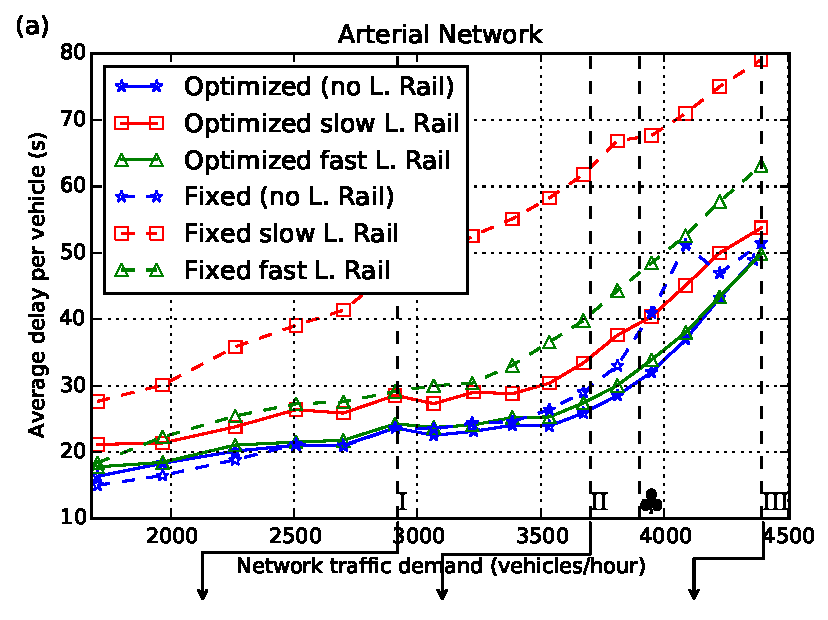
\includegraphics[keepaspectratio,height=0.3225\textwidth]{network1_delay.pdf}}
\subfigure[]{
\label{subfig:delay_3}
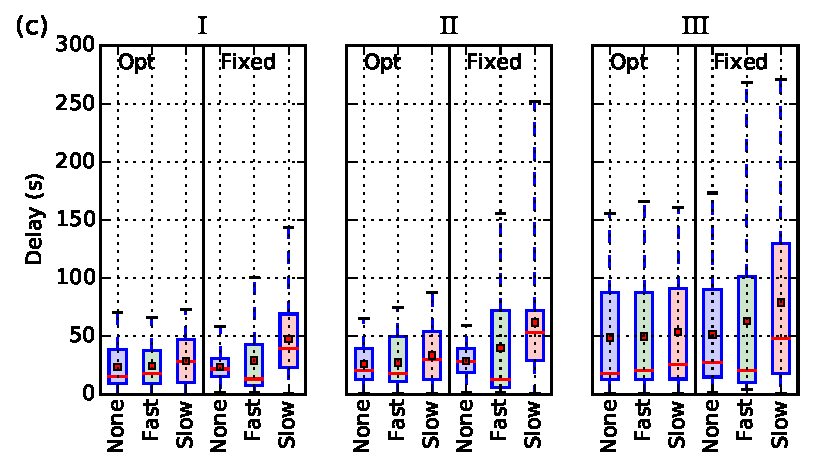
\includegraphics[keepaspectratio,height=0.3225\textwidth]{network1_boxplots.pdf}}
\caption{Increase in the total travel time w.r.t.~the optimal solution as a
function of \Nn (a,c,e) and distribution of the total delay of
each car for different values of \Nn (b,d,f).
%
For each row, the Roman numeral on top of the box plots corresponds to point the
travel time plot marked with the same numeral.
%
The mean of the total delay is presented as a red square in the box plots.
%
Plots in the $i$-th row correspond to the results for the $i$-th network in
\cref{fig:networks}.  Non-homogeneous (NH) achieves much better solutions
at smaller \Nn than Homogeneous (H).}
%control and achieves }
%smaller third quartile and maximum per-car delay for the same \Nn.}
\label{fig:results}
\end{figure*}

\begin{figure*}[t!]
\centering
%  trim={<left> <lower> <right> <upper>}
\subfigure[]{
\label{subfig:travel_time_6}
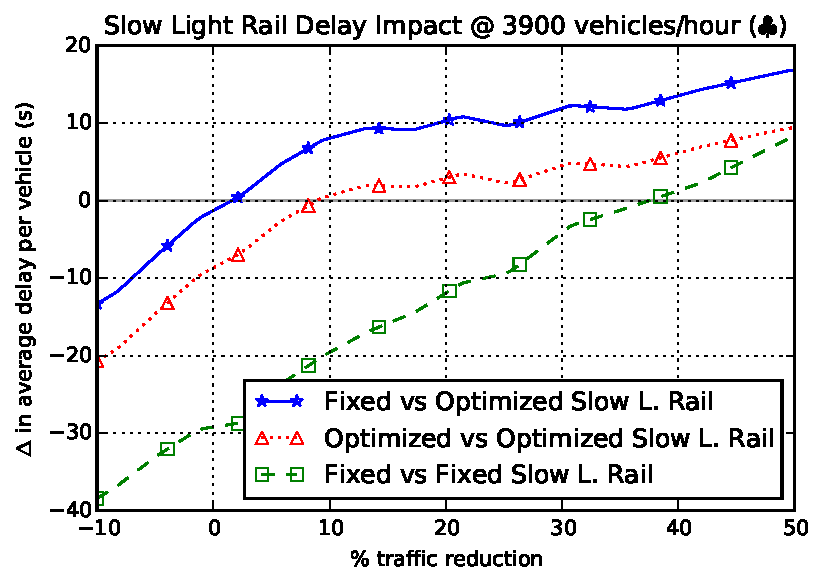
\includegraphics[keepaspectratio,height=0.3225\textwidth]{network1_t1_reduction.pdf}}
\subfigure[]{
\label{subfig:delay_6}
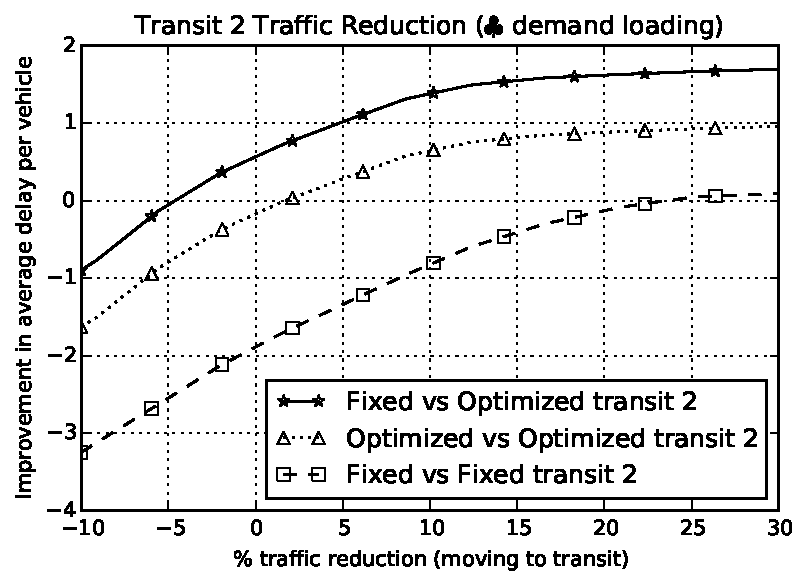
\includegraphics[keepaspectratio,height=0.3225\textwidth]{network1_t2_reduction.pdf}}
\caption{Increase in the total travel time w.r.t.~the optimal solution as a
function of \Nn (a,c,e) and distribution of the total delay of
each car for different values of \Nn (b,d,f).
%
For each row, the Roman numeral on top of the box plots corresponds to point the
travel time plot marked with the same numeral.
%
The mean of the total delay is presented as a red square in the box plots.
%
Plots in the $i$-th row correspond to the results for the $i$-th network in
\cref{fig:networks}.  Non-homogeneous (NH) achieves much better solutions
at smaller \Nn than Homogeneous (H).}
%control and achieves }
%smaller third quartile and maximum per-car delay for the same \Nn.}
\label{fig:results}
\end{figure*}

\begin{figure*}[t!]
\centering
%  trim={<left> <lower> <right> <upper>}
\subfigure[]{
\label{subfig:travel_time_9}
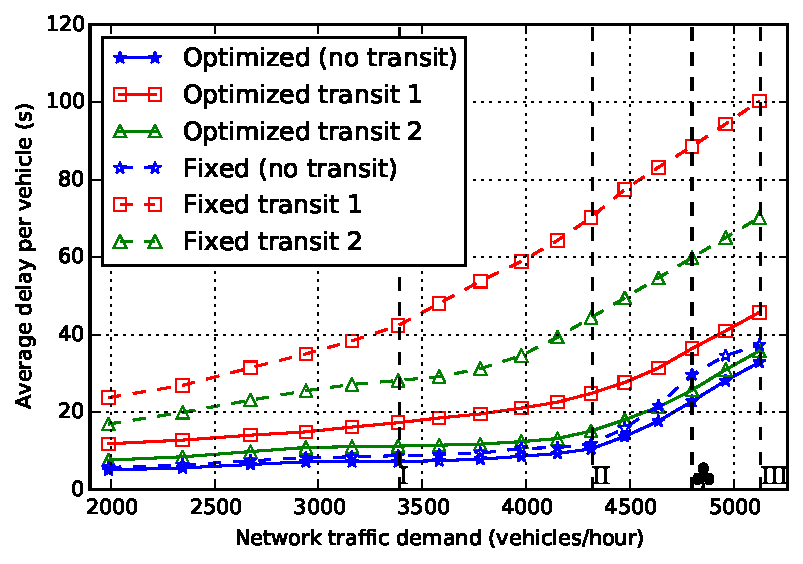
\includegraphics[keepaspectratio,height=0.3225\textwidth]{network2_delay.pdf}}
\subfigure[]{
\label{subfig:delay_9}
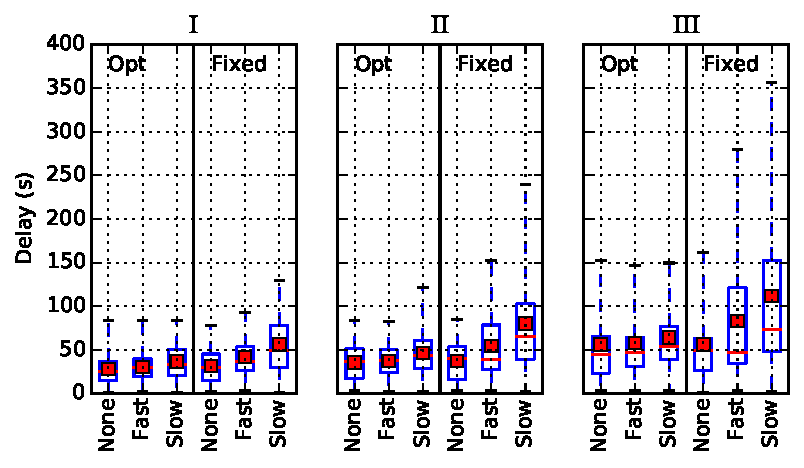
\includegraphics[keepaspectratio,height=0.3225\textwidth]{network2_boxplots.pdf}}
\caption{Increase in the total travel time w.r.t.~the optimal solution as a
function of \Nn (a,c,e) and distribution of the total delay of
each car for different values of \Nn (b,d,f).
%
For each row, the Roman numeral on top of the box plots corresponds to point the
travel time plot marked with the same numeral.
%
The mean of the total delay is presented as a red square in the box plots.
%
Plots in the $i$-th row correspond to the results for the $i$-th network in
\cref{fig:networks}.  Non-homogeneous (NH) achieves much better solutions
at smaller \Nn than Homogeneous (H).}
%control and achieves }
%smaller third quartile and maximum per-car delay for the same \Nn.}
\label{fig:results}
\end{figure*}



\begin{figure*}[t!]
\centering
%  trim={<left> <lower> <right> <upper>}
\subfigure[]{
\label{subfig:travel_time_6}
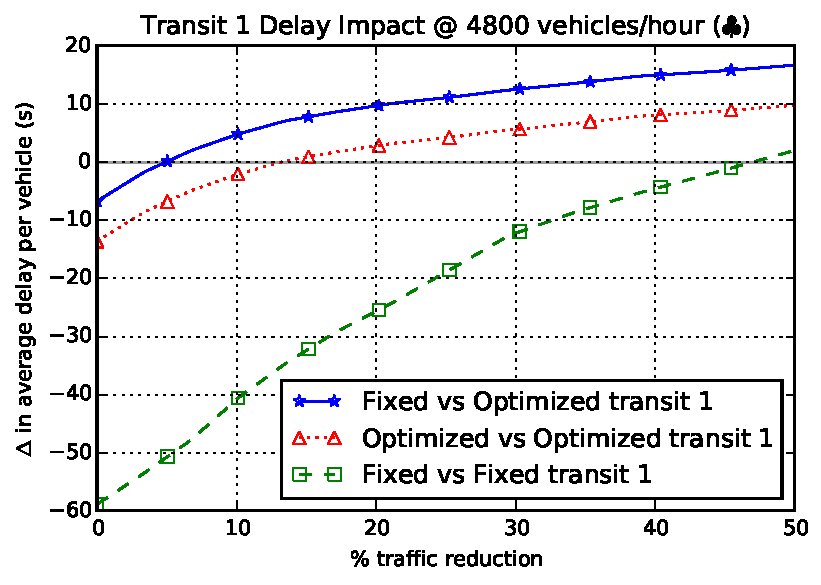
\includegraphics[keepaspectratio,height=0.3225\textwidth]{network2_t1_reduction.pdf}}
\subfigure[]{
\label{subfig:delay_6}
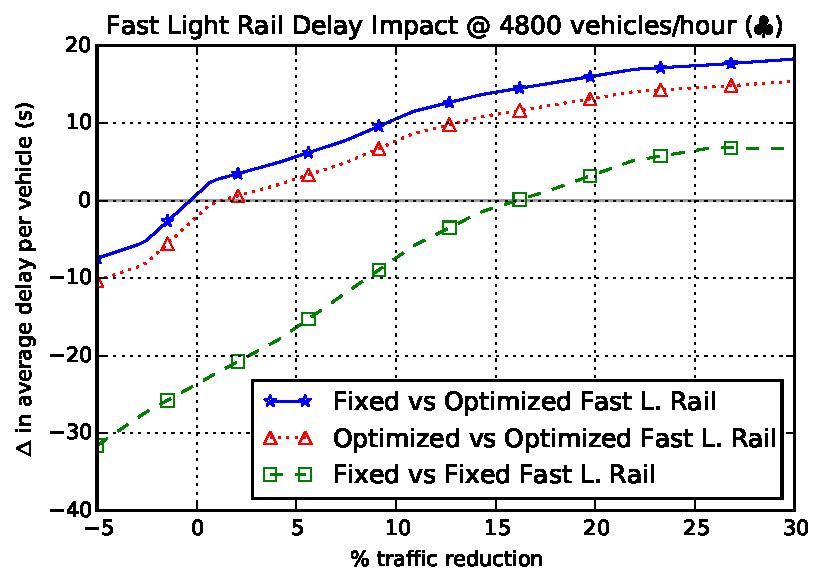
\includegraphics[keepaspectratio,height=0.3225\textwidth]{network2_t2_reduction.pdf}}
\caption{Increase in the total travel time w.r.t.~the optimal solution as a
function of \Nn (a,c,e) and distribution of the total delay of
each car for different values of \Nn (b,d,f).
%
For each row, the Roman numeral on top of the box plots corresponds to point the
travel time plot marked with the same numeral.
%
The mean of the total delay is presented as a red square in the box plots.
%
Plots in the $i$-th row correspond to the results for the $i$-th network in
\cref{fig:networks}.  Non-homogeneous (NH) achieves much better solutions
at smaller \Nn than Homogeneous (H).}
%control and achieves }
%smaller third quartile and maximum per-car delay for the same \Nn.}
\label{fig:results}
\end{figure*}


%


%We compare the performance of non-homogeneous and homogeneous solutions in two
%ways: comparing the decrease in total travel time with increasing major frame
%time (greater look ahead), and analysing the distribution of delay in each
%queue of the network.
%
\cref{subfig:travel_time_3,subfig:travel_time_6,subfig:travel_time_9} show, for
each network, the increase in the total travel time w.r.t.~the optimal solution
as a function of \Nn.
%
As we hypothesized, the non-homogeneous discretization requires less time
intervals (i.e., smaller \Nn) to obtain a solution with the same total travel
time.
%
This is important because the size of the MILP, including the number of binary
variables, scales linearly with \Nn; therefore, the non-homogeneous approach can
scale up better than the homogeneous one (e.g., \cref{subfig:travel_time_9}).
%
Also, for homogeneous and non-homogeneous discretizations, finding the optimal
solution of major frames with large \Nn might require more time than our imposed
3000s time cutoff and, in this case, Gurobi returns a feasible control plan that
is far from optimal.
%
The effect in the total travel time of these poor solutions can be seen in
\cref{subfig:travel_time_9} for $\Nn > 120$.



The distribution of the total delay observed by each car while traversing the
network is shown in \cref{subfig:delay_3,subfig:delay_6,subfig:delay_9}.
%
Each group of box plots represents a different value of~\Nn: when the
non-homogeneous $\DT[]$ first converges; when the homogeneous~$\DT[]$ first
converges; and the optimum solution itself.
%
In all networks, the quality of the solution obtained using non-homogeneous
$\DT[]$ is better or equal than using homogeneous $\DT[]$ for fixed \Nn in both
the total travel time and \emph{fairness}, i.e., smaller third quartile and
maximum delay.

%\remark{FWT: In the paragraphs above, we need to address network 2 because it is
%the exception in both cases: in the end of \cref{subfig:travel_time_6},
%homogeneous is better, and the homogeneous delay in \cref{subfig:delay_6} is
%also better.}





To further illustrate the differences between homogeneous and non-homogeneous
discretizations, \cref{fig:cumu} shows the cumulative arrival and departure
curves and the how delay evolves over time for $q_1$ of network 2
(\cref{subfig:network2}).
%
In \cref{subfig:cumu1}, the comparison is done when non-homogeneous $\DT[]$
first converges (i.e., point I in \cref{subfig:travel_time_6}) and for this
value of \Nn, the major frame size in seconds of the non-homogeneous approach is
19.125s longer than the homogeneous one.
%
This allows the MILP solver to ``see'' 19s further in the future when using
non-homogeneous discretization and find a coordinated signal policy along the
avenue to dissipate the extra traffic that arrives at time 55s.
%
The shorter major frame of the homogeneous discretization does not allow the
solver to adapt this far in advance and its delay observed after 55s is much
larger than the non-homogeneous one.
%
Once the homogeneous $\DT[]$ has converged (\cref{subfig:cumu2}), it is also
able to anticipate the increased demand and adapt well in advance and both
approaches generate solutions close to optimum (\cref{subfig:cumu3}).
